% Espansione Teorica per Algoritmi & Strutture Dati
% Da integrare nel capitolo 01_introduzione_complessita.tex

\section{Fondamenti Teorici della Complessità Computazionale}

\subsection{Teoria della Computabilità}

Prima di analizzare l'efficienza degli algoritmi, dobbiamo comprendere cosa è \textit{computabile}. La teoria della computabilità studia i limiti fondamentali del calcolo.

\begin{tcolorbox}[colback=blue!10, colframe=blue!60, title=Definizione: Computabilità]
Un problema è \textbf{computabile} (o \textit{decidibile}) se esiste un algoritmo che, dato un input qualsiasi, termina sempre fornendo la risposta corretta in un numero finito di passi.
\end{tcolorbox}

\textbf{Esempi di problemi non computabili}:

\begin{enumerate}
    \item \textbf{Problema della Fermata (Halting Problem)}: Dato un programma $P$ e un input $I$, determinare se $P$ terminerà o continuerà all'infinito.

    \item \textbf{Problema della Corrispondenza di Post}: Determinare se esiste una sequenza di "tessere" che produce stringhe identiche sopra e sotto.

    \item \textbf{Problema del Decimo di Hilbert}: Determinare se un'equazione diofantea ha soluzioni intere.
\end{enumerate}

\begin{tcolorbox}[colback=yellow!10, colframe=orange!60, title=Teorema: Indecidibilità del Problema della Fermata]
\textbf{Teorema} (Turing, 1936): Non esiste un algoritmo generale che, dato un programma arbitrario e un input, possa determinare se il programma terminerà.

\textbf{Dimostrazione} (per assurdo):

Supponiamo esista un algoritmo $H(P, I)$ che decide se il programma $P$ termina con input $I$:
\[
H(P, I) = \begin{cases}
\text{TERMINA} & \text{se } P \text{ termina con input } I \\
\text{LOOP} & \text{se } P \text{ va in loop con input } I
\end{cases}
\]

Costruiamo ora un programma paradossale $D$:

\begin{lstlisting}[caption=Programma Diagonale D]
def D(P):
    if H(P, P) == TERMINA:
        loop_infinito()  # Va in loop
    else:
        return  # Termina
\end{lstlisting}

Cosa succede se eseguiamo $D(D)$?
\begin{itemize}
    \item Se $H(D, D) =$ TERMINA, allora $D(D)$ va in loop $\rightarrow$ contraddizione
    \item Se $H(D, D) =$ LOOP, allora $D(D)$ termina $\rightarrow$ contraddizione
\end{itemize}

Quindi $H$ non può esistere. $\square$
\end{tcolorbox}

\subsection{Classi di Complessità: P vs NP}

\subsubsection{La Classe P}

\begin{tcolorbox}[colback=green!10, colframe=green!60, title=Definizione: Classe P]
La classe \textbf{P} (Polynomial Time) contiene tutti i problemi decisionali risolvibili da un algoritmo deterministico in tempo polinomiale rispetto alla dimensione dell'input.

Formalmente: $P = \bigcup_{k=1}^{\infty} \text{TIME}(n^k)$
\end{tcolorbox}

\textbf{Esempi di problemi in P}:
\begin{itemize}
    \item Ordinamento di $n$ elementi: $O(n \log n)$
    \item Ricerca binaria: $O(\log n)$
    \item Cammino minimo (Dijkstra): $O(V^2)$ o $O((V+E) \log V)$
    \item Albero di copertura minimo (Kruskal/Prim): $O(E \log V)$
    \item Matching massimo in grafi bipartiti: $O(V^3)$
\end{itemize}

\subsubsection{La Classe NP}

\begin{tcolorbox}[colback=green!10, colframe=green!60, title=Definizione: Classe NP]
La classe \textbf{NP} (Nondeterministic Polynomial Time) contiene tutti i problemi decisionali per cui, data una soluzione candidata, è possibile \textit{verificare} la correttezza in tempo polinomiale.

Equivalentemente: problemi risolvibili da una macchina di Turing non deterministica in tempo polinomiale.
\end{tcolorbox}

\textbf{Esempi di problemi in NP}:
\begin{itemize}
    \item \textbf{SAT (Soddisfacibilità Booleana)}: Data una formula booleana, esiste un'assegnazione di valori che la rende vera?

    \item \textbf{CLIQUE}: Dato un grafo $G$ e un intero $k$, esiste una clique di dimensione $k$?

    \item \textbf{Commesso Viaggiatore (TSP)}: Esiste un tour che visita tutte le città con costo $\leq k$?

    \item \textbf{Knapsack}: Esiste un sottoinsieme di oggetti con valore totale $\geq k$ e peso $\leq W$?

    \item \textbf{Colorazione Grafi}: È possibile colorare un grafo con $k$ colori senza nodi adiacenti dello stesso colore?
\end{itemize}

\textbf{Perché sono in NP?} Perché se qualcuno ci fornisce una soluzione candidata (es: assegnazione di variabili per SAT), possiamo verificarla in tempo polinomiale.

\subsubsection{P = NP? Il Problema del Millennio}

\begin{tcolorbox}[colback=red!10, colframe=red!60, title=La Domanda Fondamentale]
\textbf{P = NP?}

Questa è una delle domande più importanti dell'informatica teorica (Millennium Prize Problem da 1 milione di dollari).

\begin{itemize}
    \item Se \textbf{P = NP}: Verificare una soluzione è facile $\Rightarrow$ Trovarla è altrettanto facile
    \item Se \textbf{P $\neq$ NP}: Esistono problemi dove verificare è facile, ma trovare la soluzione è difficile
\end{itemize}

\textbf{Consenso scientifico}: La maggior parte degli informatici ritiene che P $\neq$ NP, ma non esiste ancora una dimostrazione.
\end{tcolorbox}

\subsubsection{Problemi NP-Completi}

\begin{tcolorbox}[colback=purple!10, colframe=purple!60, title=Definizione: NP-Completezza]
Un problema $X$ è \textbf{NP-Completo} se:
\begin{enumerate}
    \item $X \in$ NP
    \item Per ogni problema $Y \in$ NP, esiste una riduzione polinomiale $Y \leq_P X$
\end{enumerate}

In altre parole: sono i problemi "più difficili" in NP. Se risolvi efficientemente un problema NP-Completo, hai risolto tutti i problemi NP!
\end{tcolorbox}

\textbf{Teorema di Cook-Levin} (1971): SAT è NP-Completo.

\textbf{Catena di riduzioni}:
\[
\text{SAT} \leq_P \text{3-SAT} \leq_P \text{CLIQUE} \leq_P \text{VERTEX-COVER} \leq_P \text{SUBSET-SUM}
\]

\begin{figure}[h]
\centering
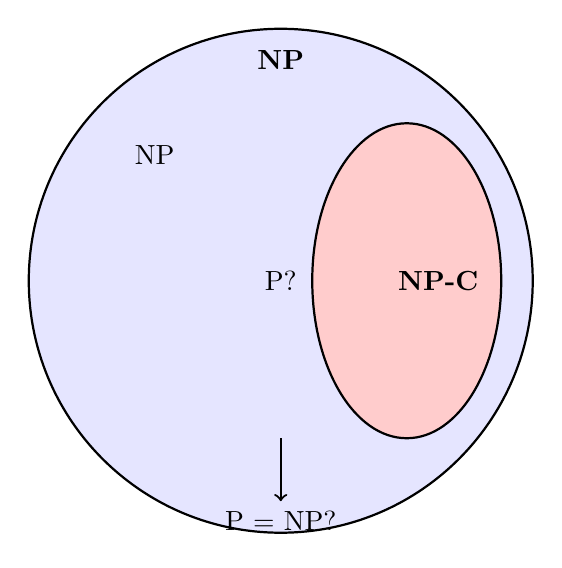
\begin{tikzpicture}[scale=0.8]
    % P circle
    \draw[thick, fill=green!20] (0,0) circle (2cm);
    \node at (0,-1.2) {\textbf{P}};

    % NP circle
    \draw[thick, fill=blue!10] (0,0) circle (4cm);
    \node at (0,3.5) {\textbf{NP}};

    % NP-Complete region
    \draw[thick, fill=red!20] (2,0) ellipse (1.5cm and 2.5cm);
    \node at (2.5,0) {\textbf{NP-C}};

    % Labels
    \node at (-2,2) {NP};
    \node at (0,0) {P?};

    % Question mark
    \draw[thick, ->] (0,-2.5) -- (0,-3.5) node[below] {P = NP?};
\end{tikzpicture}
\caption{Relazione tra le classi di complessità (ipotesi P $\neq$ NP)}
\end{figure}

\subsection{Analisi Amortizzata}

L'analisi amortizzata studia il costo \textit{medio} di una sequenza di operazioni, non il worst-case di singole operazioni.

\subsubsection{Metodo del Potenziale}

\begin{tcolorbox}[colback=cyan!10, colframe=cyan!60, title=Tecnica: Analisi Amortizzata con Potenziale]
Definiamo una funzione potenziale $\Phi(D_i)$ che rappresenta l'"energia accumulata" nella struttura dati dopo $i$ operazioni.

Il costo ammortizzato dell'operazione $i$ è:
\[
\hat{c}_i = c_i + \Phi(D_i) - \Phi(D_{i-1})
\]

Dove:
\begin{itemize}
    \item $c_i$ = costo reale dell'operazione $i$
    \item $\Phi(D_i)$ = potenziale dopo operazione $i$
    \item $\hat{c}_i$ = costo ammortizzato
\end{itemize}
\end{tcolorbox}

\textbf{Esempio: Dynamic Array con Raddoppiamento}

Consideriamo un array dinamico che raddoppia la capacità quando è pieno.

\begin{itemize}
    \item \textbf{Operazione normale}: Inserimento in $O(1)$
    \item \textbf{Raddoppiamento}: Copia di $n$ elementi in $O(n)$
\end{itemize}

\textbf{Analisi worst-case}: $O(n)$ per singola operazione.

\textbf{Analisi ammortizzata}: Definiamo $\Phi(D_i) = 2n_i - c_i$ dove:
\begin{itemize}
    \item $n_i$ = numero elementi
    \item $c_i$ = capacità array
\end{itemize}

Costo ammortizzato inserimento:
\begin{align*}
\hat{c}_i &= c_i + (2n_i - c_i) - (2n_{i-1} - c_{i-1}) \\
&= 1 + 2 = 3 = O(1)
\end{align*}

Quindi $n$ inserimenti costano $O(n)$ ammortizzato!

\subsection{Lower Bounds Teorici}

Non tutti i problemi possono essere risolti arbitrariamente veloce. Esistono \textbf{lower bounds} fondamentali.

\subsubsection{Lower Bound per l'Ordinamento Basato su Confronti}

\begin{tcolorbox}[colback=orange!10, colframe=orange!60, title=Teorema: Lower Bound Ordinamento]
\textbf{Teorema}: Qualsiasi algoritmo di ordinamento basato su confronti richiede $\Omega(n \log n)$ confronti nel caso peggiore per ordinare $n$ elementi.

\textbf{Dimostrazione}:

L'albero di decisione per $n$ elementi ha:
\begin{itemize}
    \item Foglie: $n!$ (permutazioni possibili)
    \item Altezza: numero massimo di confronti
\end{itemize}

Un albero binario di altezza $h$ ha al massimo $2^h$ foglie:
\[
2^h \geq n! \implies h \geq \log_2(n!) = \Omega(n \log n)
\]

Usando l'approssimazione di Stirling: $n! \approx \sqrt{2\pi n} \left(\frac{n}{e}\right)^n$

Quindi: $\log(n!) \approx n \log n - n \log e = \Theta(n \log n)$ $\square$
\end{tcolorbox}

\textbf{Conseguenza}: Merge Sort e Heap Sort sono ottimi asintoticamente!

\subsubsection{Lower Bounds per Problemi Specifici}

\begin{itemize}
    \item \textbf{Ricerca in array non ordinato}: $\Omega(n)$ (devi guardare tutti gli elementi)
    \item \textbf{Moltiplicazione matrici}: $\Omega(n^2)$ (devi leggere l'input)
    \item \textbf{Convex Hull in 2D}: $\Omega(n \log n)$ (riduzione da ordinamento)
    \item \textbf{Element Uniqueness}: $\Omega(n \log n)$ (sotto decision tree model)
\end{itemize}

\subsection{Invarianti e Correttezza degli Algoritmi}

\subsubsection{Invarianti di Ciclo}

\begin{tcolorbox}[colback=violet!10, colframe=violet!60, title=Definizione: Invariante di Ciclo]
Un \textbf{invariante di ciclo} è una proprietà che:
\begin{enumerate}
    \item \textbf{Inizializzazione}: È vera prima della prima iterazione
    \item \textbf{Mantenimento}: Se è vera prima dell'iterazione $k$, rimane vera prima dell'iterazione $k+1$
    \item \textbf{Terminazione}: Quando il ciclo termina, l'invariante fornisce una proprietà utile che dimostra la correttezza
\end{enumerate}
\end{tcolorbox}

\textbf{Esempio: Insertion Sort}

\textbf{Invariante}: All'inizio dell'iterazione $j$, il sottoarray $A[1..j-1]$ contiene gli elementi originali di $A[1..j-1]$ ma ordinati.

\textbf{Dimostrazione di correttezza}:

\begin{itemize}
    \item \textbf{Inizializzazione} ($j=2$): $A[1..1]$ ha un solo elemento, quindi è trivialmente ordinato. ✓

    \item \textbf{Mantenimento}: Assumiamo $A[1..j-1]$ ordinato. Il corpo del ciclo inserisce $A[j]$ nella posizione corretta di $A[1..j]$, quindi $A[1..j]$ diventa ordinato. ✓

    \item \textbf{Terminazione}: Il ciclo termina quando $j = n+1$. L'invariante implica che $A[1..n]$ (l'intero array) è ordinato. ✓
\end{itemize}

\subsubsection{Funzioni di Terminazione}

Per dimostrare che un algoritmo termina, usiamo una \textbf{funzione di terminazione} $f$:

\begin{enumerate}
    \item $f$ mappa lo stato del programma in un insieme ben ordinato (es: $\mathbb{N}$)
    \item $f$ decresce strettamente ad ogni iterazione
    \item $f \geq 0$ sempre
\end{enumerate}

\textbf{Esempio: Binary Search}

Funzione di terminazione: $f = \text{right} - \text{left}$

\begin{itemize}
    \item Inizialmente: $f = n - 0 = n$
    \item Ad ogni iterazione: intervallo dimezzato, quindi $f$ decresce
    \item Quando $f = 0$: $\text{left} = \text{right}$, l'algoritmo termina
\end{itemize}

\subsection{Tecniche Avanzate di Analisi}

\subsubsection{Master Theorem Esteso}

Il Master Theorem risolve ricorrenze della forma:
\[
T(n) = aT(n/b) + f(n)
\]

\begin{tcolorbox}[colback=gray!10, colframe=black!60, title=Master Theorem - Forma Generale]
Siano $a \geq 1$ e $b > 1$ costanti, e sia $f(n)$ una funzione asintoticamente positiva.

Definiamo $n_{\text{crit}} = \log_b a$ (esponente critico).

\begin{enumerate}
    \item Se $f(n) = O(n^c)$ con $c < n_{\text{crit}}$: $T(n) = \Theta(n^{n_{\text{crit}}})$

    \item Se $f(n) = \Theta(n^{n_{\text{crit}}} \log^k n)$ per $k \geq 0$: $T(n) = \Theta(n^{n_{\text{crit}}} \log^{k+1} n)$

    \item Se $f(n) = \Omega(n^c)$ con $c > n_{\text{crit}}$ e $af(n/b) \leq kf(n)$ per $k < 1$: $T(n) = \Theta(f(n))$
\end{enumerate}
\end{tcolorbox}

\textbf{Applicazioni}:

\begin{itemize}
    \item \textbf{Merge Sort}: $T(n) = 2T(n/2) + \Theta(n)$
    \begin{align*}
    a=2, b=2, f(n)=n \\
    n_{\text{crit}} = \log_2 2 = 1 \\
    f(n) = \Theta(n^1 \log^0 n) \implies T(n) = \Theta(n \log n)
    \end{align*}

    \item \textbf{Karatsuba}: $T(n) = 3T(n/2) + \Theta(n)$
    \begin{align*}
    n_{\text{crit}} = \log_2 3 \approx 1.585 \\
    f(n) = O(n^1), \quad 1 < 1.585 \implies T(n) = \Theta(n^{1.585})
    \end{align*}
\end{itemize}

\section*{Conclusione}

Questi fondamenti teorici forniscono le basi per comprendere non solo "come" funzionano gli algoritmi, ma anche "perché" alcuni problemi sono intrinsecamente difficili e quali sono i limiti fondamentali del calcolo.

La teoria della complessità ci insegna che:
\begin{itemize}
    \item Non tutti i problemi sono computabili
    \item Tra quelli computabili, alcuni richiedono tempo esponenziale
    \item Esistono lower bounds teorici invalicabili
    \item L'analisi ammortizzata rivela costi "nascosti"
\end{itemize}

Questi concetti sono essenziali per ogni informatico serio e verranno ripresi nei capitoli successivi con applicazioni concrete.
